\documentclass[11pt]{article}

% some definitions for the title page
\newcommand{\reporttitle}{example}
\newcommand{\reportdescription}{example description}

% load some definitions and default packages
%---------------------------------------------------------------------------
%	PACKAGES AND OTHER DOCUMENT CONFIGURATIONS
%---------------------------------------------------------------------------

\usepackage[twoside]{fancyhdr}
\usepackage{csquotes}

\usepackage[a4paper,hmargin=2.0cm,vmargin=1.0cm,includeheadfoot]{geometry}
% \usepackage{natbib} % for bibliography
\usepackage{biblatex}
\usepackage{tabularx,longtable,multirow,subfigure,caption}%hangcaption
\usepackage{fancyhdr} % page layout
\usepackage{url} % URLs
\usepackage[english]{babel}
\usepackage{graphicx}
\usepackage{rotating}
\usepackage{dsfont}
\usepackage{epstopdf} % automatically replace .eps with .pdf in graphics
% \usepackage{backref} % needed for citations
\usepackage{array}
\usepackage{latexsym}
\usepackage[pdftex,hypertexnames=false,colorlinks]{hyperref} % provide links in pdf (had pagebackref)
\usepackage{booktabs}
\usepackage{wrapfig}
\usepackage{caption}  % Required for \captionof
\usepackage{float} % for H option in figures
\usepackage{amssymb}
\usepackage{amsmath}
\usepackage{amsthm}
\usepackage{mathtools} % for 'dcases*' env.
\usepackage[nottoc]{tocbibind}

%%% Default fonts
\renewcommand*{\rmdefault}{bch}
\renewcommand*{\ttdefault}{cmtt}

%%% Default settings (page layout)
\setlength{\parindent}{0em}  % indentation of paragraph
\setlength{\parskip}{.3em}
\setlength{\itemsep}{0.mm}

\setlength{\headheight}{14.5pt}
\pagestyle{fancy}

\fancyfoot[ER,OL]{\thepage}%Page no. in the left on odd pages and on right on even pages

\fancyfoot[OC,EC]{\sffamily }
\renewcommand{\headrulewidth}{0.1pt}
\renewcommand{\footrulewidth}{0.1pt}
\captionsetup{margin=10pt,font=small,labelfont=bf}

% LISTINGS ammendments
\usepackage{listings}
\usepackage{color}

\definecolor{mygreen}{rgb}{0,0.6,0}
\definecolor{mygray}{rgb}{0.5,0.5,0.5}
\definecolor{mymauve}{rgb}{0.58,0,0.82}

\lstset{ 
  postbreak=\mbox{\textcolor{red}{$\hookrightarrow$}\space},
  backgroundcolor=\color{white},   % choose the background color; you must add \usepackage{color} or \usepackage{xcolor}; should come as last argument
  basicstyle=\footnotesize,        % the size of the fonts that are used for the code
  breakatwhitespace=false,         % sets if automatic breaks should only happen at whitespace
  breaklines=true,                 % sets automatic line breaking
  captionpos=b,                    % sets the caption-position to bottom
  commentstyle=\color{mygreen},    % comment style
%   deletekeywords={...},            % if you want to delete keywords from the given language
%   escapeinside={\%*}{*)},          % if you want to add LaTeX within your code
  extendedchars=true,              % lets you use non-ASCII characters; for 8-bits encodings only, does not work with UTF-8
  firstnumber=1,                % start line enumeration with line 1000
  frame=single,	                   % adds a frame around the code
  keepspaces=true,                 % keeps spaces in text, useful for keeping indentation of code (possibly needs columns=flexible)
  columns=fullflexible,
  keywordstyle=\color{blue},       % keyword style
  language=python,                 % the language of the code
  % morekeywords={*,...},            % if you want to add more keywords to the set
  numbers=left,                    % where to put the line-numbers; possible values are (none, left, right)
  numbersep=5pt,                   % how far the line-numbers are from the code
  numberstyle=\tiny\color{mygray}, % the style that is used for the line-numbers
  rulecolor=\color{black},         % if not set, the frame-color may be changed on line-breaks within not-black text (e.g. comments (green here))
  showspaces=false,                % show spaces everywhere adding particular underscores; it overrides 'showstringspaces'
  showstringspaces=false,          % underline spaces within strings only
  showtabs=false,                  % show tabs within strings adding particular underscores
  stepnumber=1,                    % the step between two line-numbers. If it's 1, each line will be numbered
  stringstyle=\color{mymauve},     % string literal style
  tabsize=2,	                   % sets default tabsize to 2 spaces
  title=\lstname% show the filename of files included with \lstinputlisting; also try caption instead of title
}

% Here, you can define your own macros. Some examples are given below.

\newcommand{\R}[0]{\mathds{R}} % real numbers
\newcommand{\Z}[0]{\mathds{Z}} % integers
\newcommand{\N}[0]{\mathds{N}} % natural numbers
\newcommand{\C}[0]{\mathds{C}} % complex numbers
\renewcommand{\vec}[1]{{\boldsymbol{{#1}}}} % vector
\newcommand{\mat}[1]{{\boldsymbol{{#1}}}} % matrix


\begin{document}

% Include the title page
\begin{titlepage}

    \newcommand{\HRule}{\rule{\linewidth}{0.5mm}} % Defines a new command for the horizontal lines, change thickness here
    
    \center % Center everything on the page
     
    %------------------------------------------------------------------------
    %	HEADING SECTIONS
    %------------------------------------------------------------------------
    
    \textsc{\Large Department of Computing}\\[0.5cm] 
    \textsc{\large Imperial College of Science, Technology and Medicine}\\[0.5cm] 
    
    %------------------------------------------------------------------------
    %	TITLE SECTION
    %------------------------------------------------------------------------
    
    \HRule \\[0.4cm]
    { \huge \bfseries \reporttitle}\\ % Title of your document
    \HRule \\[0.4cm]

    \textit{\reportdescription}
    
    \vspace{2em}

    %------------------------------------------------------------------------
    %	AUTHOR SECTION
    %------------------------------------------------------------------------
    
    \large \emph{Author: Anton Zhitomirskiy}

    \vspace{1em}

    \global\let\newpagegood\newpage
    \global\let\newpage\relax
    
\end{titlepage}

\global\let\newpage\newpagegood

\tableofcontents

\clearpage

\section{NLP Classification tasks}

\begin{definition}[Classification]
    \begin{equation}
        \hat{y} = \arg\max_y P(y|x)    
    \end{equation}
    Predicting which `class' an observation belongs to
\end{definition}

A Model produces a score (logit), a sigmoid makes this between 0 and 1, and 0.5 is our decision boundary. In multi-class classification we then use softmax.

\subsection{Natural Language Inference}

a model is presented with a pair of sentences and must classify the relationship between their meanings. For example in the MultiNLI corpus, pairs of sentences are given one of 3 labels: entails, contradicts and neutral. These labels describe a relationship between the meaning of the first sentence (the premise) and the meaning of the second sentence (the hypothesis). Here are representative examples of each class from the corpus:

\begin{itemize}
    \item \textbf{Premise}: The kitten is climbing the curtains again
    \item \textbf{Hypothesis}: The kitten is sleeping
    \item \textbf{Entailment}: If the hypothesis is implied by the premise
    \item \textbf{Contradiction}: If the hypothesis contradicts the premise (in this example, the hypothesis is contradicting)
    \item \textbf{Neutral}: otherwise (neither is necessarily true)
\end{itemize}

\section{Naive Bayes}

(Generative Algorithm)

\begin{definition}[Bayes Rule]
    \begin{equation*}
        \underbrace{P(y|x)}_\text{Posterior} = \frac{\overbrace{P(x|y)}^\text{Likelihood}\overbrace{P(y)}^\text{Prior}}{\underbrace{P(x)}_\text{Evidence}}
    \end{equation*}
\end{definition}

Since $P(x)$ won't change for different classes

\begin{warning}
    why?
\end{warning}

\begin{equation*}
    \hat{y} = \arg \max_y P(y|x) = \arg \max_y P(x|y)P(y)
\end{equation*}

We can further state that since $x$ is a set of features $x_1, \ldots, x_I$ we have a independence assumption:

\begin{definition}[Naiive Bayes Classifier]\label{eq:naiive-bayes-classifier}
    \begin{align*}
        & P(x_1, \ldots, x_I|y)=P(x_1|y) \cdots P(x_I|y) \\
        \hat{y} = \arg \max_y & P(x_1, \ldots, x_I|y)P(y) = \arg \max_y P(y) \prod ^ I _{i=1} P(x_i|y)
    \end{align*}
\end{definition}

\subsection{Add-one smoothing}

Raw input is transformed into a numerical representation - i.e. each input $x$ is represented by a feature vector by using a Bag of Words approach (count of each word in the input)
``This was another good movie for holiday watchers. There was a nice little twist at the end''
\begin{table}[h]
    \centering
    \begin{tabular}{|c|c|c|c|c|c|c|c|}
        \hline
        & \textbf{a} & \textbf{about} & \textbf{another} & \textbf{and} & \textbf{$\cdots$} & \textbf{was} & \textbf{you} \\
        \hline
        Review \#1 & 1 & 0 & 1 & 0 & & 2 & 0 \\
        \hline
    \end{tabular}
\end{table}
Collect statistics from our training data (find what $P(y|x)$ is) after performing limited data-preprocessing.

\begin{figure}[H]
    \centering
    \includegraphics*[width=\linewidth]{figures/example.png}
    \caption{Example of training corpus. Here, we are only concerned with the words `good', `movie', and `bad' for classes `+' and `-'}
\end{figure}

\begin{align*}
    P(y) & \rightarrow P(+) = \frac 3 5, \quad P(-) = \frac 2 5 \\ 
    P(good|+) & = \frac 2 4 & \text{i.e. } \frac{\text{frequency of word for class}}{\text{total count of words for this class}}
\end{align*}

this introduces the problem that one of our probabilities could be zero; therefore, adjust naive bayes classifier with `Add-one smoothing'

\begin{definition}[Add-one smoothing]\label{eq:add-one-smoothing}
    \begin{equation*}
        P(x_i|y) = \frac{count(x_i,y)+1}{\sum_{x\in V}(count(x,y)+1)} = \frac{count(x_i, y) + 1}{(\sum_{x\in V} count(x,y)) + |V|}
    \end{equation*}
\end{definition}

\begin{align*}
    P(good|+) = \frac {2 + 1} {4 + 3} = \frac 3 7 & P(good|-) = \frac{1 + 1}{3 + 3} = \frac 2 6 \\
    P(movie|+) = \frac{1 + 1}{4 + 3} = \frac 2 7  & P(movie|-) = \frac{1 + 1}{3 + 3} = \frac 2 6  \\
    P(bad|+) = \frac{1 + 1}{4 + 3} = \frac 2 7  & P(bad|-) = \frac{1 + 1}{3 + 3} = \frac 2 6
\end{align*} 

Therefore for a test example: ``Not as \textbf{good} as the old \textbf{movie}, rather \textbf{bad}'' we use Equation~\ref{eq:naiive-bayes-classifier} to get $P(+)P(x|+) = \frac 3 5 \times \frac{3\times 2 \times 2}{7^3} = 0.021$ and $P(-)P(x|-) = \frac 2 5 \times \frac{2\times 2 \times 2}{6^3} = 0.014$. So final outcome of the model is $+$. However, this sentence is clearly negative, yet we classify as positive.

\subsection{Binary Naive Bayes}

Within binary naive bayes, we only consider if a feature is present, rather than considering every time it occurs. Note, this means re-calculating the conditional probabilities from the training data.

E.g. ``Not as \textbf{good} as the old \textbf{movie}, rather \textbf{bad movie}'' we have $P(+)P(x|+) = \frac 3 5 \times \frac{3\times 2 \times 2}{7^3} = 0.021$ and $P(-)P(x|-) = \frac 2 5 \times \frac{2 \times 2 \times 2}{6^3} = 0.014$. If we were still operating under the same formula in Equation~\ref{eq:naiive-bayes-classifier} then we would have iterated over the label `movie' twice, and thus multiplied by $P(good|+)$ twice (in the positive case).

\subsection{Controlling for negation}

We append `Not\_' after any logical negation (e..g n't, not, no, never) until the next punctuation mark.

``I didn't like the movie, but it was better than Top Gun'' becomes ``I didn't NOT\_like NOT\_the NOT\_movie, but it was better than Top Gun''

\subsection{Problems}

\begin{itemize}
    \item Conditional independence assumption
    \item Features considered equally important
    \item Context of words not taken into account
    \item New words (not seen at training) cannot be used
\end{itemize}

\subsection{Summary}

Very quick to train, Some evidence it works well on very small datasets.

\section{Logistic Regression}

(Discriminative Algorithm) because we directly learn $P(Y|X)$ since we don't care about $P(Y)$ or $P(X)$. They learn the input feauters most useful to discriminate between the different classes, without considering the likelihood of the input itself.

\begin{align*}
    y(x) & = g(z) = \frac 1 {1 + e^{-z}} \\
    z & = w \cdot x + b \\
    P(y=1) & = \frac{1 } {1 + e^{- (w \cdot x + b)}}
\end{align*}

where $w$ is how important an input feature is to the classification decision and we have a threshold at 0.5 for decision making.

\begin{figure}[H]
    \centering
    \includegraphics*[width=.6\linewidth]{figures/example2.png}
\end{figure}

If we don't have the w, then we learn parameters to make the model predictions close to our labels by using a loss function (to measure the distance between the true and predicted labels) and optimization algorithm (to minimize the function usually through gradient descent.)

\begin{definition}[Logistic Regression]
    \begin{equation*}
        H(P,Q) = -\sum_i P(y_i)\log Q(y_i)
    \end{equation*}
\end{definition}

\subsection{Multiple Classes}

Weights and bias are learnt per class, then use a softmax function over the result of finding $z_i$.

\begin{equation*}
    y=g(z_i)=\frac{e^{z_i}}{\sum^k_{j=1}e^{z_j}}
\end{equation*}

\subsection{Summary}

Logistic Regression considers the importance of feautres, so is better (than Naive Bayes) at dealing with correlated feautres, also better (than Naive Bayes) with larger datasets.

\section{Neural Networks (NNs)}

\begin{definition}[Linear Layer]
    \begin{equation*}
        z = w \cdot x + b = \sum^I_{i=0}w_ix_i + b
    \end{equation*}
\end{definition}

\begin{definition}[Non-linear activation function]
    \begin{equation*}
        y = g(z)
    \end{equation*}
\end{definition}

\begin{definition}[Fully-connected layers]
    \begin{equation*}
        FFN(x) = (g^2(g^1(xW^1+b^1))W^2 + b^2)W^3 + b^3
    \end{equation*}
\end{definition}

The neural networks allow for automatically learning dense feature representations, not one-hot encodings.

\subsection{Docuemnt Representation}

How to get a document representation of sentence of
fixed dimensionality?

Average of sentence - bad idea:
    
Model architecutre fixed to sentence length size, model wieghts learnt for specific word positions

\subsection{Neural Networks}

Automatically learned features; flexibility to fit highly complex relationships in data, but they require more data to learn more complex patterns.

\section{Recurrent neural networks (RNNs)}

\begin{figure}[H]
    \centering
    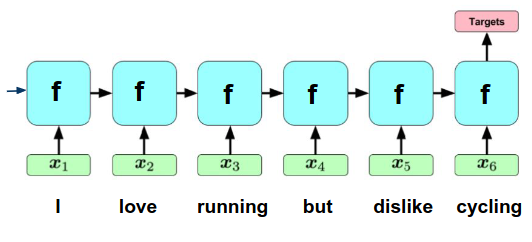
\includegraphics[width=.6\linewidth]{figures/RNN.png}    
\end{figure}

Natural language data is made up of sequences, so its natural to represent in a RNN; the value of a unit depends on own previous outputs - the last hidden state is the input to the output layer.

\begin{figure}[H]
    \centering
    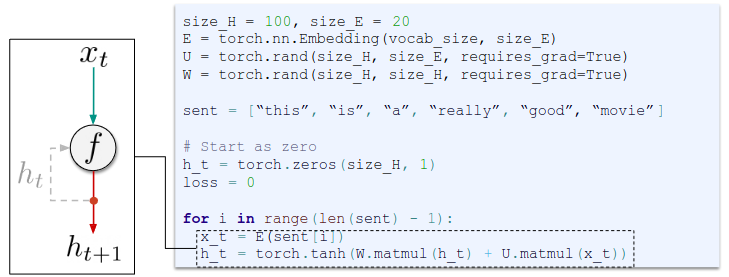
\includegraphics[width=.6\linewidth]{figures/VanillaRNN.png}    
\end{figure}

\subsection{Vanishing gradient problem}

The model is less able to learn from earlier inputs (Tanh derivatives are between 0 and 1) (Sigmoid derivatives are between 0 and 0.25) - Gradient for earlier layers involves repeated multiplication
of the same matrix W - depending on the dominant eignevalue this can cause gradients to either `vanish' or `explode'

\begin{warning}
    RNNs perform better when you need to understand longer range dependencies
\end{warning}

\section{CNNs}

CNNs are composed of a series of convolution layers,
pooling layers and fully connected layers. Convolutional layers Detect important patterns in the inputs. Pooling layers Reduce dimensionality of features and transform them into a fixed-size. Fully connected layers Train weights of learned representation for a specific task.

We can stack multiple filters on-top of eachother also.

\begin{warning}
    CNNs can perform well if the task involves key phrase recognition.
\end{warning}

\section{Accuracy and F1}

\begin{definition}[accuracy]
    \begin{equation*}
        Accuracy = \frac{TP + TN}{TP +FP + TN + FN}
    \end{equation*}
\end{definition}

\begin{definition}[f1-measure]
    \begin{equation*}
        f1 = 2 \times \frac{precision\times recall}{precision + recall} = \frac{TP}{TP + 0.5 (FP +FN)}
    \end{equation*}
\end{definition}

\subsection{Macro averaging}

averaging of each class F1 scores: increases the emphasis on less frequent classes

\subsection{Micro averaging}

TPs, TNs,  FNs. FPs are summed across each class.

Microaveraged F1

\begin{figure}[H]
    \centering
    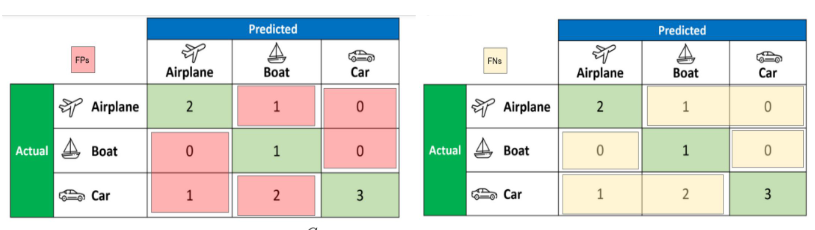
\includegraphics[width=.6\linewidth]{figures/f1.png}    
\end{figure}

\begin{equation*}
    \frac{\sum^C_i TP_i}{\sum^C_i TP_i + 0.5 (\sum^C_i FP_i + \sum^C_i FN_i)} = \frac{\sum^C_i TP_i}{|Dataset|} = Accuracy
\end{equation*}

\end{document}